\documentclass{article}

\usepackage{caption}
\usepackage{subcaption}
\usepackage{amsmath}
\usepackage{url}

\usepackage{arxiv}

\usepackage[utf8]{inputenc} % allow utf-8 input
\usepackage[T1]{fontenc}    % use 8-bit T1 fonts
\usepackage{hyperref}       % hyperlinks
\usepackage{url}            % simple URL typesetting
\usepackage{booktabs}       % professional-quality tables
\usepackage{amsfonts}       % blackboard math symbols
\usepackage{nicefrac}       % compact symbols for 1/2, etc.
\usepackage{microtype}      % microtypography
\usepackage{lipsum}
\usepackage{graphicx}
\graphicspath{ {./images/} }


\title{CRISPR Screen}

\author{Margaux Failla \\
	\And 
	Keira Wiechecki \\
	\And 
	Lionel Christiaen \\
}
\date{\today}

\begin{document}

\section{Results}

\begin{figure}
	\caption{}
	\label{fig:}
\end{figure}

\begin{figure}
     \begin{subfigure}[b]{0.4\textwidth}
         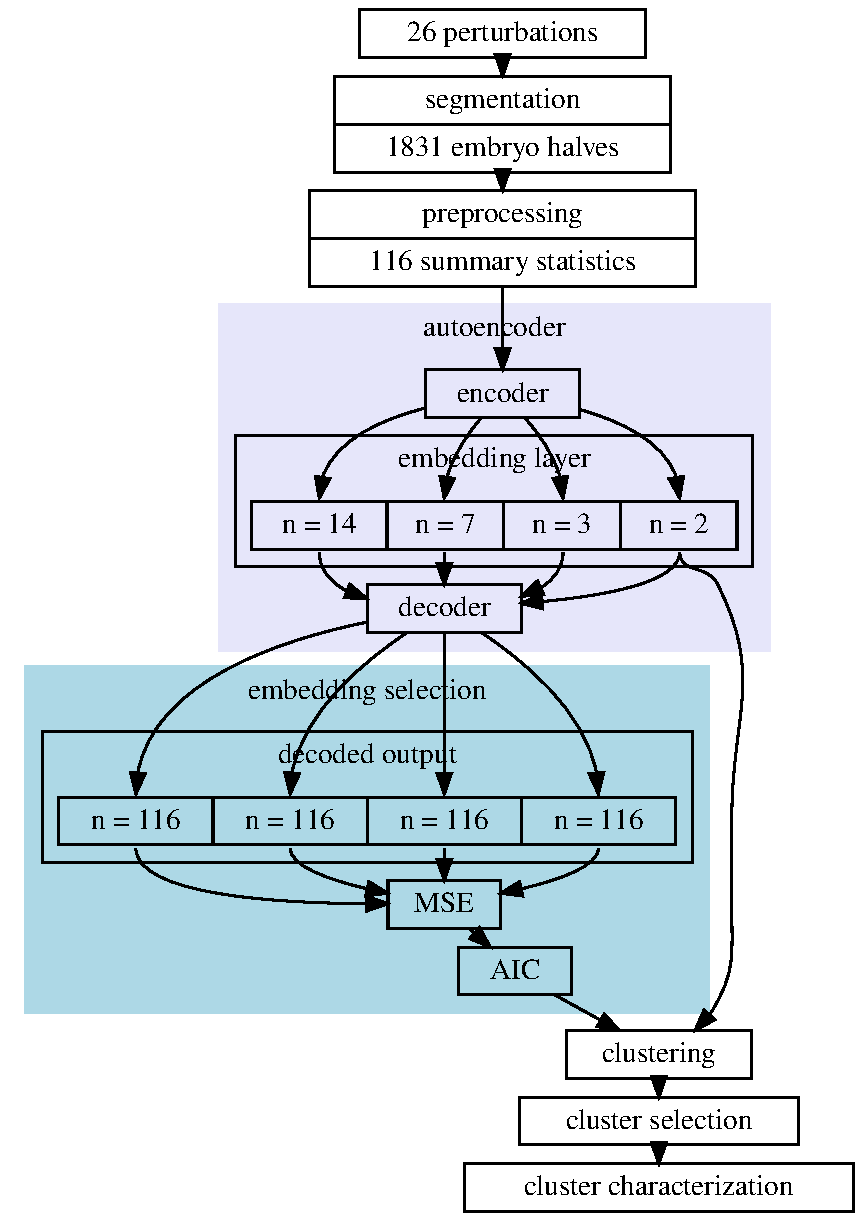
\includegraphics[width=\textwidth]{encode.dot.pdf}
         \caption{}
         \label{fig:}
     \end{subfigure}
     \hfill
%     \begin{subfigure}[b]{0.5\textwidth}
%         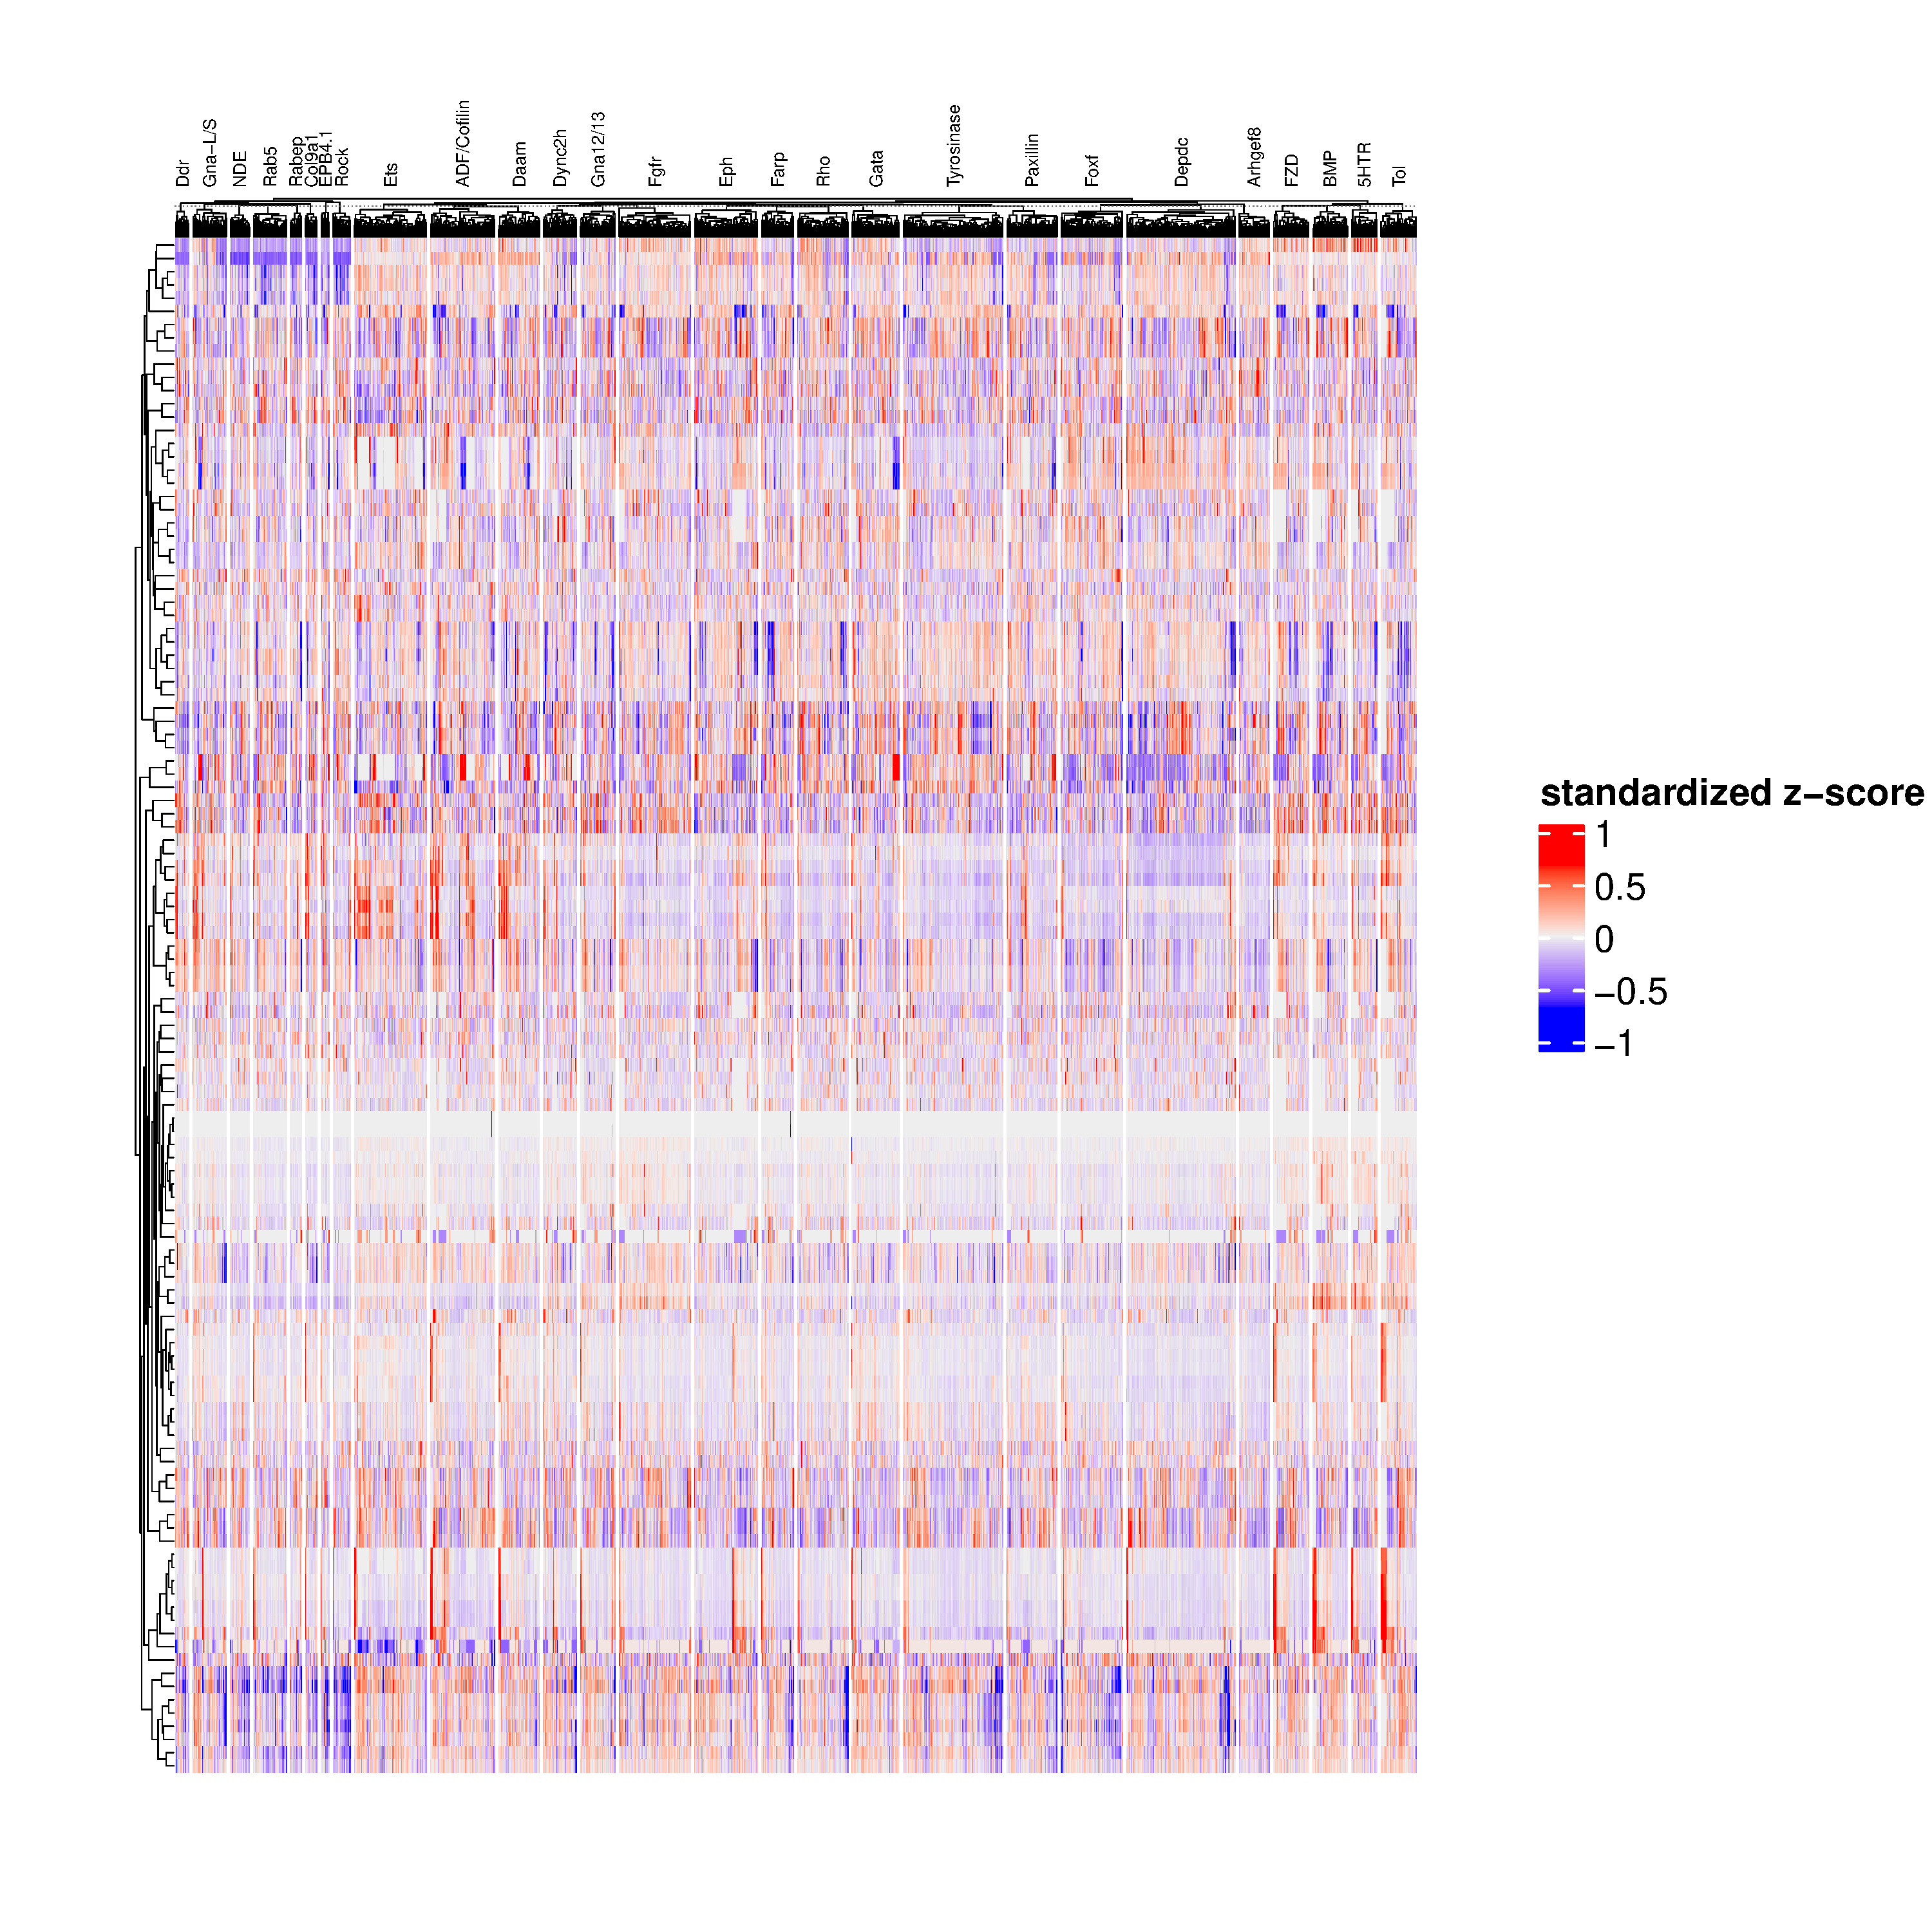
\includegraphics[width=\textwidth]{params.pdf}
%         \caption{}
%         \label{fig:}
%     \end{subfigure}
%     \vspace{1cm}
     \begin{subfigure}[b]{0.6\textwidth}
         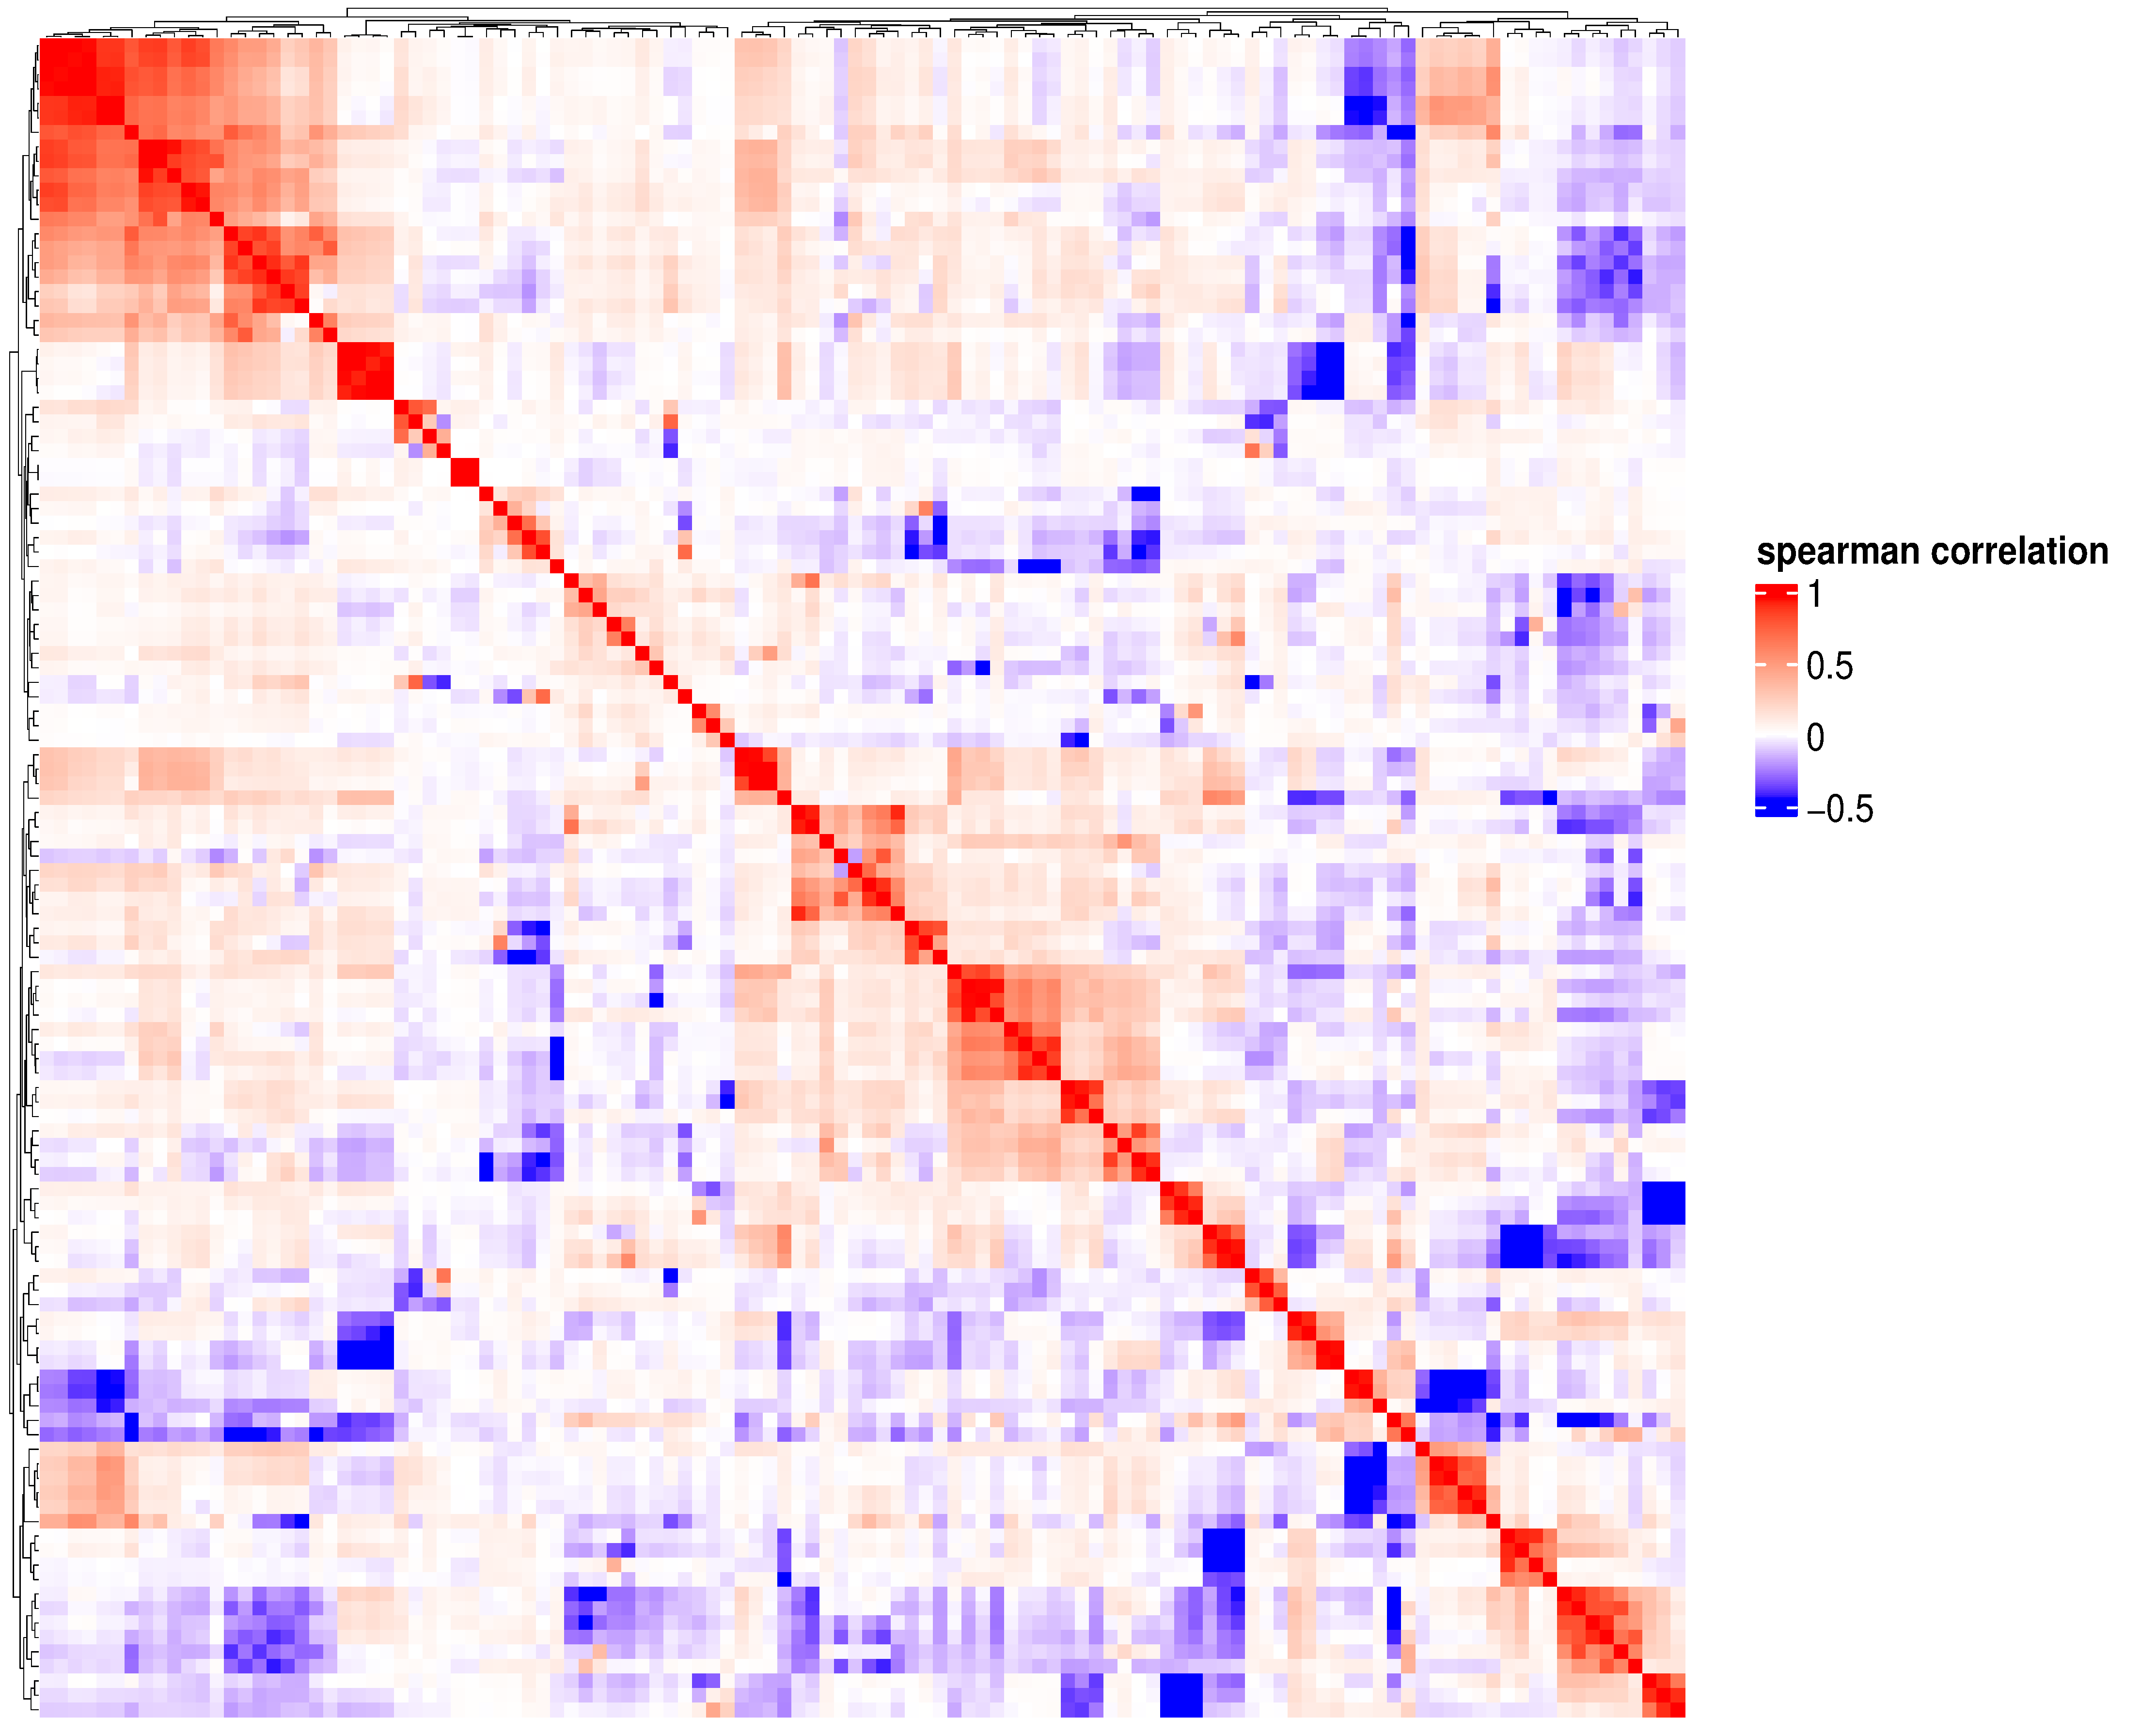
\includegraphics[width=\textwidth]{correlation.pdf}
         \caption{}
         \label{fig:}
     \end{subfigure}
     \vspace{1cm}
     \begin{subfigure}[b]{0.5\textwidth}
         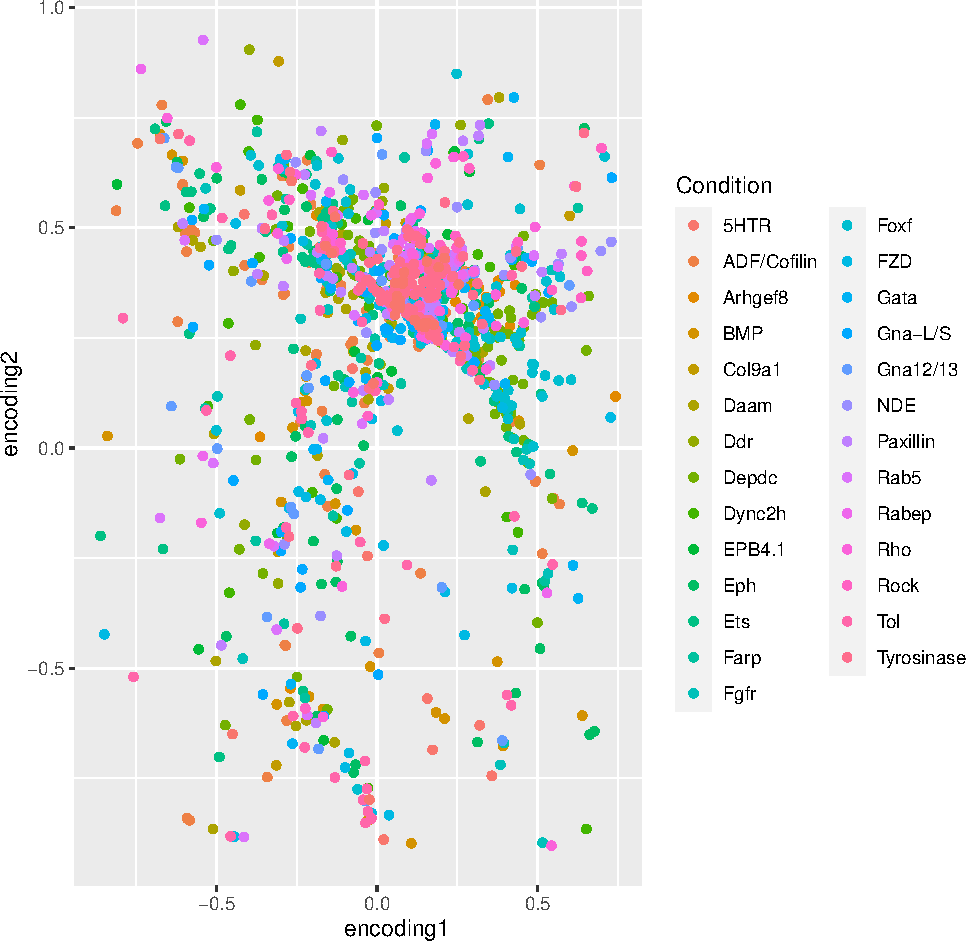
\includegraphics[width=\textwidth]{embedding.cond.pdf}
         \caption{}
         \label{fig:}
     \end{subfigure}
     \hfill
     \begin{subfigure}[b]{0.5\textwidth}
         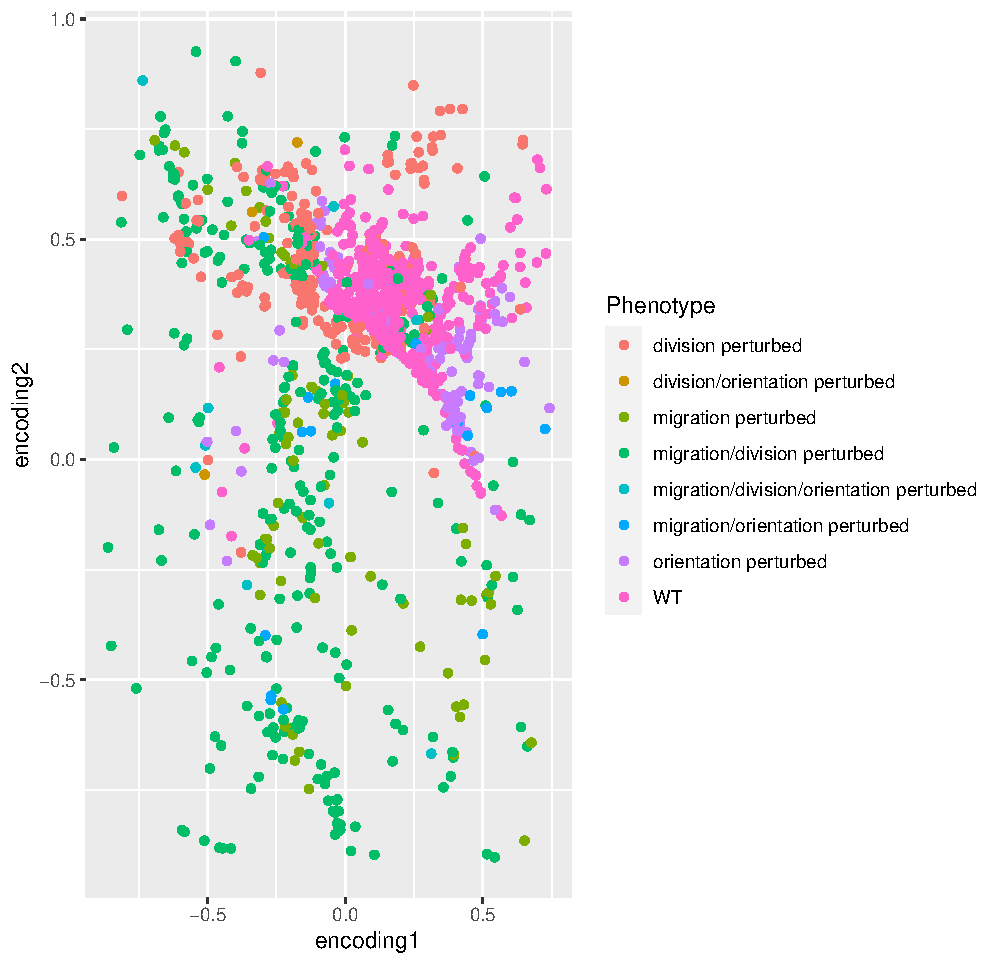
\includegraphics[width=\textwidth]{embedding.pheno.pdf}
         \caption{}
         \label{fig:}
     \end{subfigure}
\caption{(a) Workflow for embedding selection. Four autoencoders were run in parallel with output embedding dimensions $n \in \{2,3,7,14\}$. We used AIC to select an embedding as described in equation (1).  
(b) Spearman correlation of input parameters to autoencoder. 
(c) Embedding values for 2 dimensions by experimental perturbation.
(d) Embedding values by experimenter-labeled phenotype.}
\label{fig:}
\end{figure}

\begin{table}
	\centering
\begin{tabular}{|c|c|c|c|}
	\hline
	dimension of embedding layer & number of layers & MSE & AIC \\
	\hline
2 & 12 & 0.018663 & 4.03 \\
3 & 10 & 0.015585 & 6.03 \\
7 & 8 & 0.010944 & 14.02 \\
14 & 6 & 0.006231 & 28.01 \\
\hline
\end{tabular}
\caption{MSE and AIC values for each model. A low MSE means the model is better able to recreate the data. A lower AIC indicates adding more embedding dimensions improves MSE sub-logarithmically.}
\end{table}

\begin{figure}
	\begin{subfigure}[b]{0.4\textwidth}
		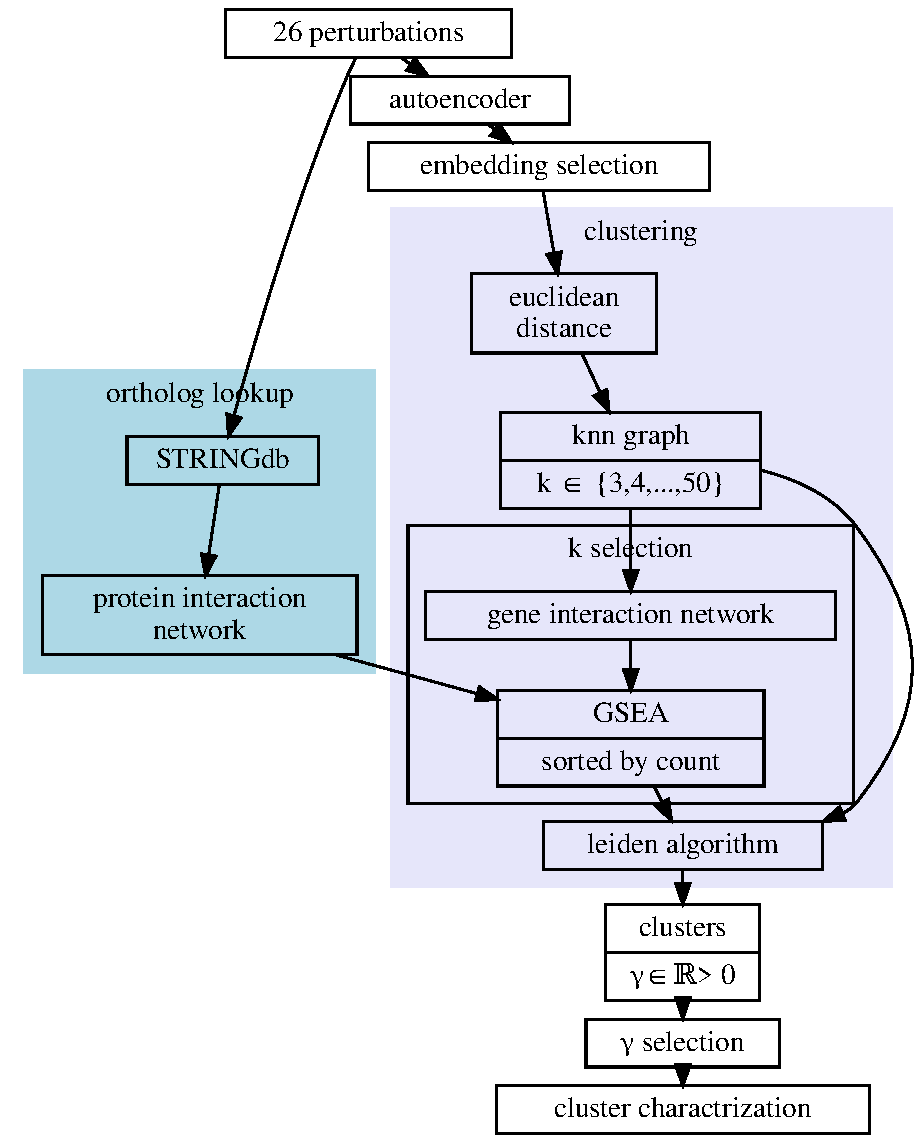
\includegraphics[width=\textwidth]{cluster.dot.pdf}
		\caption{}
		\label{fig:}
	\end{subfigure}
	\begin{subfigure}[b]{0.2\textwidth}
		\begin{subfigure}[b]{\textwidth}
			\includegraphics[width=\textwidth]{es.pdf}

			\caption{}
			\label{}
		\end{subfigure}
		\begin{subfigure}[b]{\textwidth}
			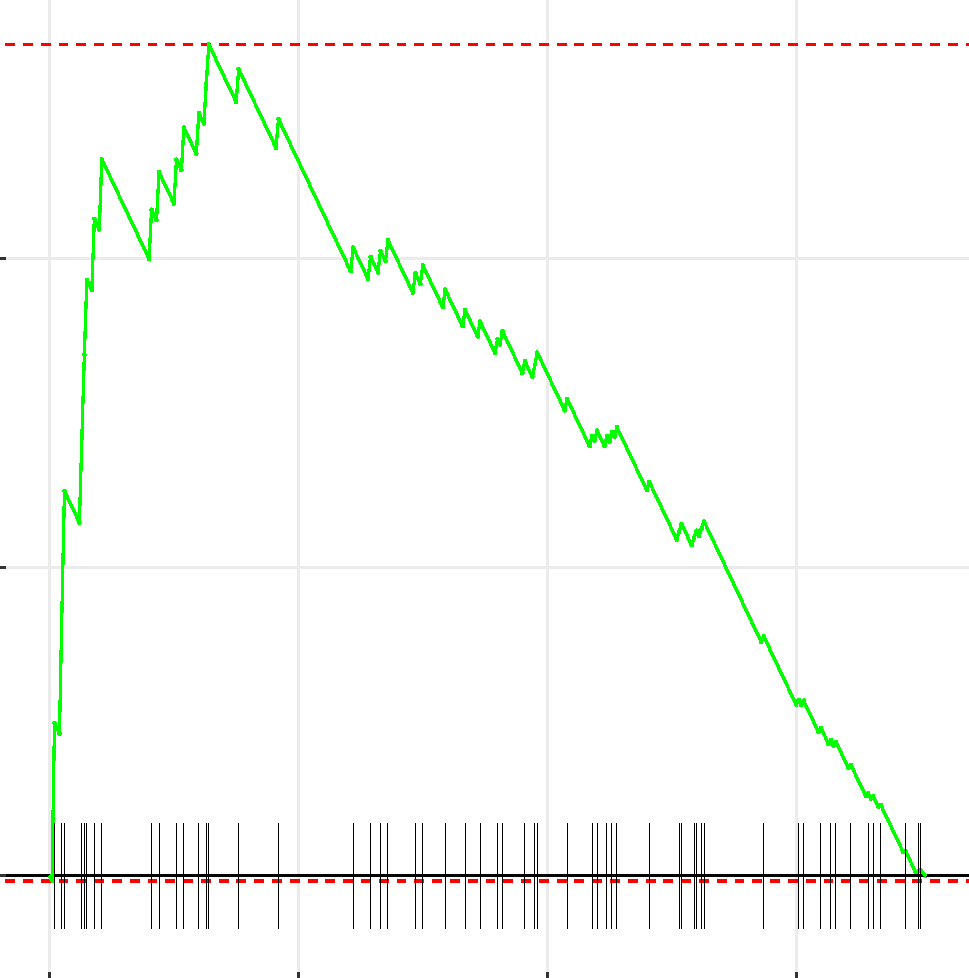
\includegraphics[width=\textwidth]{interaction_enrichment.pdf}

			\caption{}
			\label{}
		\end{subfigure}
		

	\end{subfigure} 
	\begin{subfigure}[b]{0.4\textwidth}
		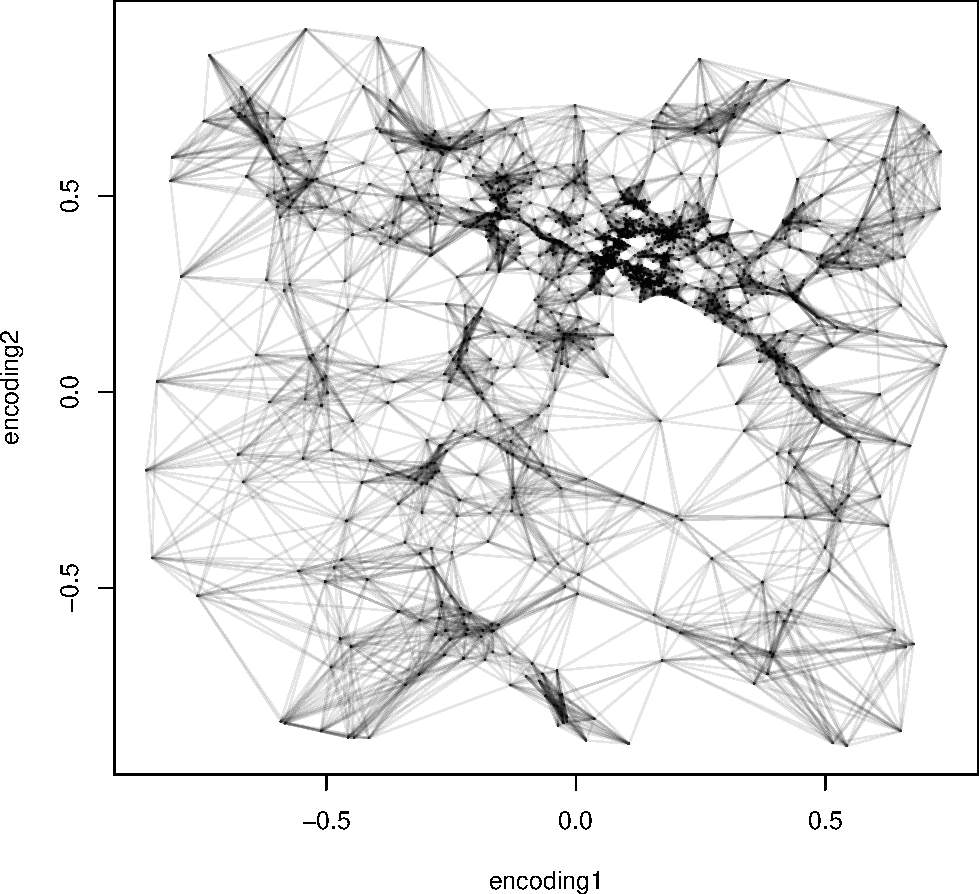
\includegraphics[width=\textwidth]{knn.pdf}

		\caption{}
		\label{}

	\end{subfigure} 
	\vspace{1cm}
	\begin{subfigure}[b]{0.5\textwidth}
		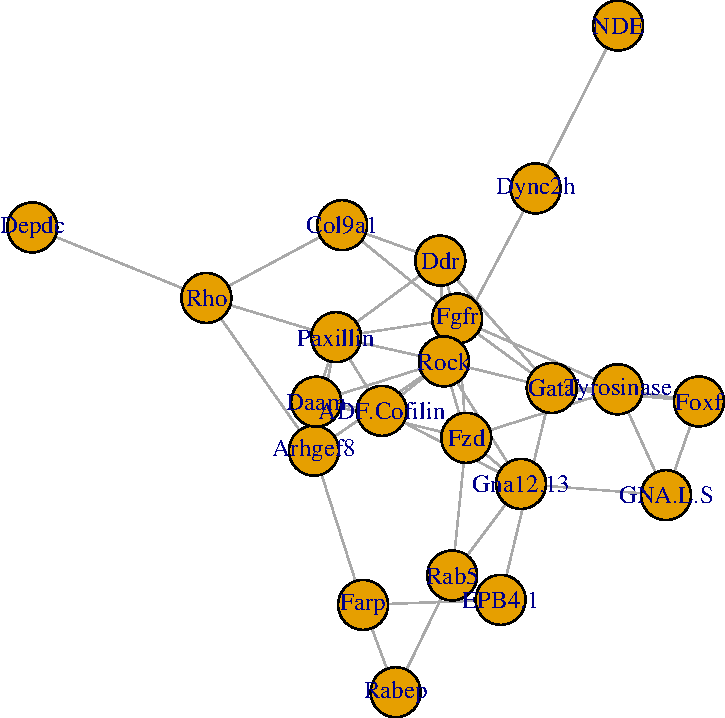
\includegraphics[width=\textwidth]{interactions.pdf}
		\caption{}
		\label{}
	\end{subfigure}
	\hfill
	\begin{subfigure}[b]{0.5\textwidth}
		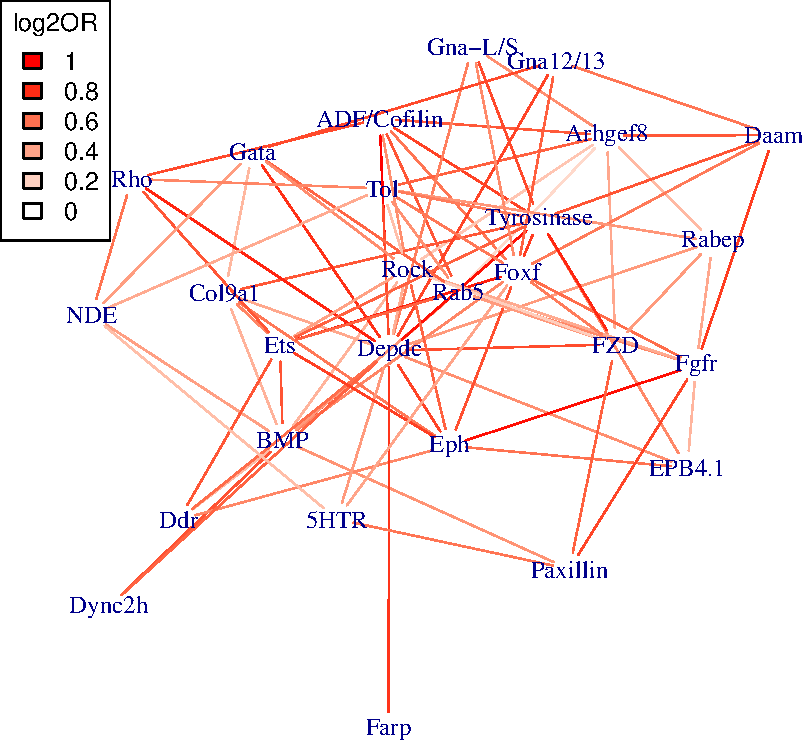
\includegraphics[width=\textwidth]{hyper.k.pdf}
		\caption{}
		\label{}
	\end{subfigure}
%	\begin{subfigure}[b]{0.3\textwidth}
%		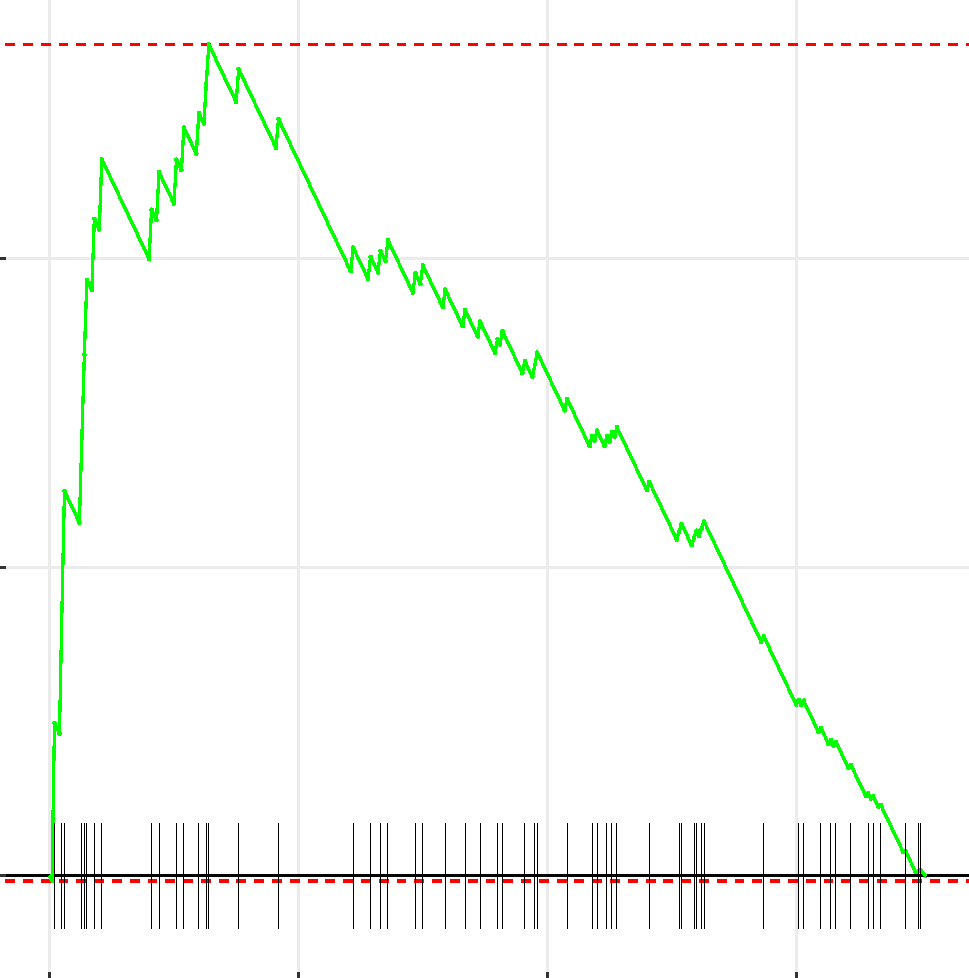
\includegraphics[width=\textwidth]{interaction_enrichment.pdf}
%		\caption{}
%		\label{}
%	\end{subfigure}
%	\hfill
	\caption{(a) Workflow for clustering embryos. 
	(b) Enrichment scores for $k$ between 3 and 53.
(c) Example enrichment score calculation. The $x$-axis gives gene pairs ranked by number of edges in a $k$-NN for a given $k$. The $y$-axis gives the running enrichment score, which is incremented when a pair corresponds to a known interaction and decremented if not. The maximum value gives the output enrichment score, resulting in a higher score the more concentrated known interactions are to the top of the list. 
(d) 17-NN graph of embryos.
(e) Protein interaction network obtained from STRINGdb.
(f) Gene interaction network obtained from enrichment of edges in (d) as described in equation (3). The $log2(OR)$ shows the overrepresentation of edges between pairs of conditions compared to a uniform distribution of edges beween conditions as described in equation (4).}
	\label{}

\end{figure}


\begin{figure}
	\begin{subfigure}[b]{0.5\textwidth}
		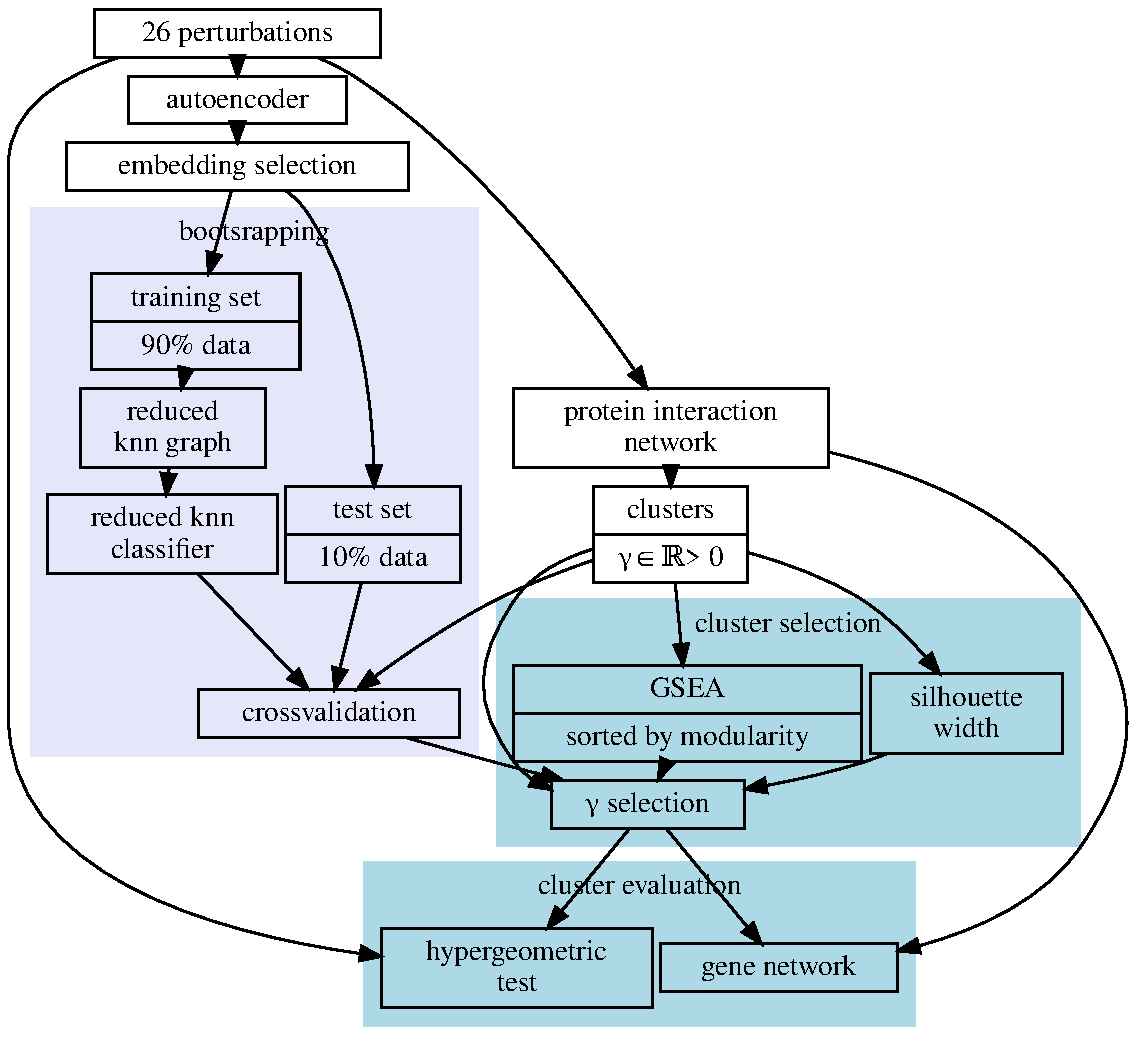
\includegraphics[width=\textwidth]{sel.dot.pdf}
		\caption{}
		\label{fig:}
	\end{subfigure}
	\hfill
	\begin{subfigure}[b]{0.5\textwidth}
		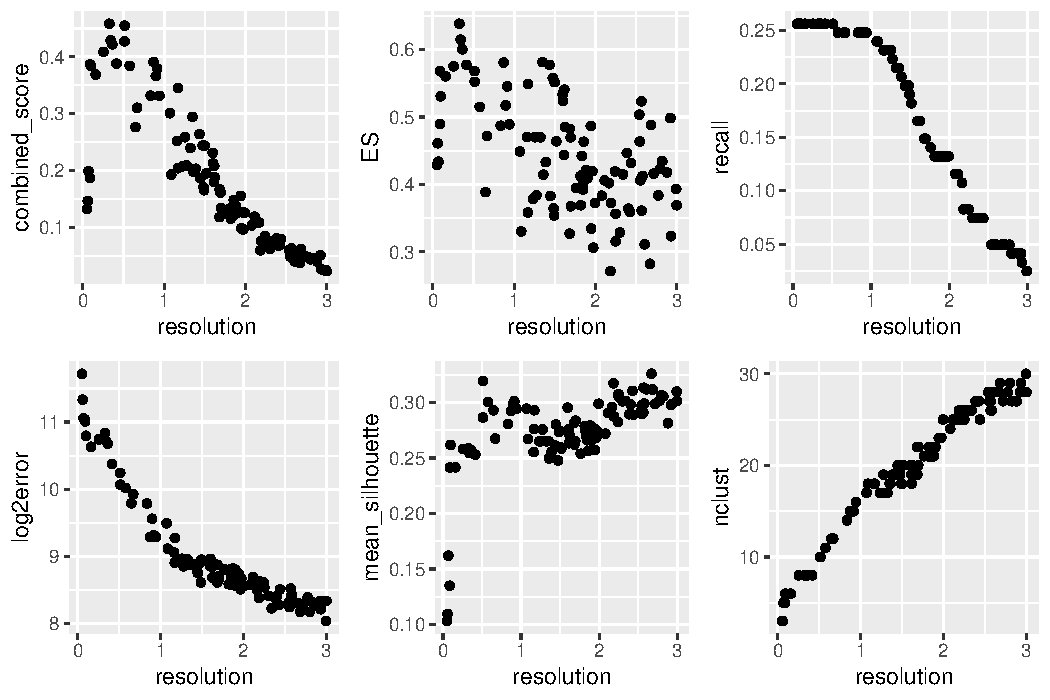
\includegraphics[width=\textwidth]{leiden.k17.optimization.pdf}

		\caption{}
		\label{}

	\end{subfigure} 
	\vspace{1cm}
	\begin{subfigure}[b]{0.37\textwidth}
		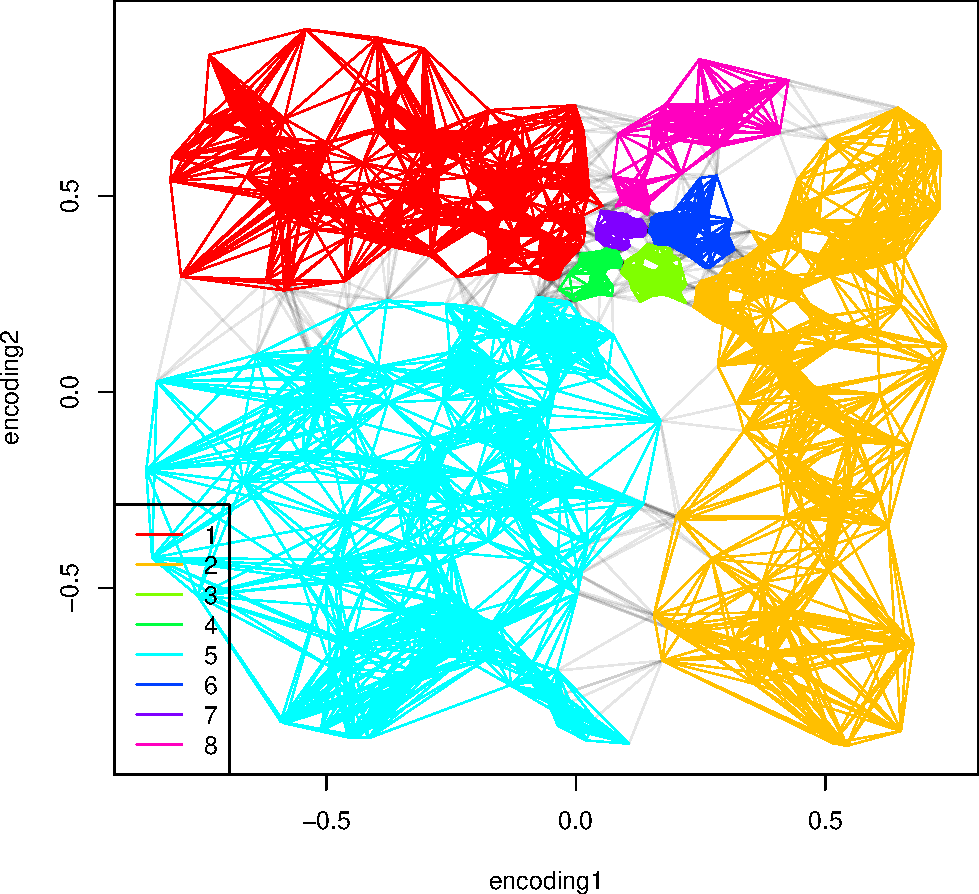
\includegraphics[width=\textwidth]{knn.clust.pdf}
		\caption{}
		\label{}
	\end{subfigure}
	\hfill
	\begin{subfigure}[b]{0.25\textwidth}
		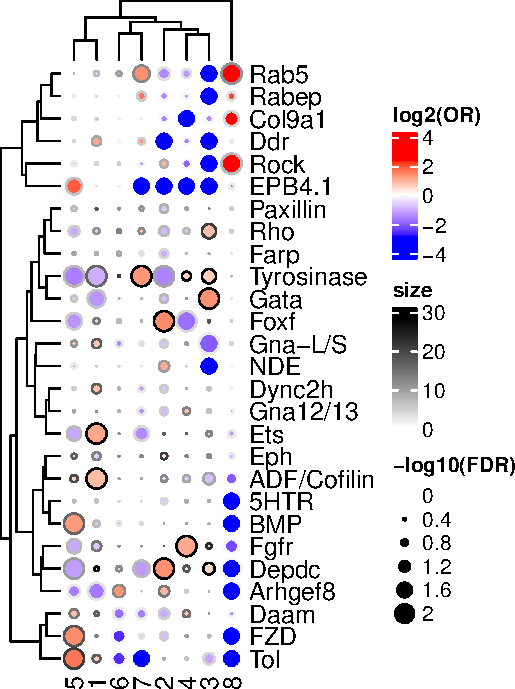
\includegraphics[width=\textwidth]{condition.pdf}
		\caption{}
		\label{}
	\end{subfigure}
	\hfill
	\begin{subfigure}[b]{0.37\textwidth}
		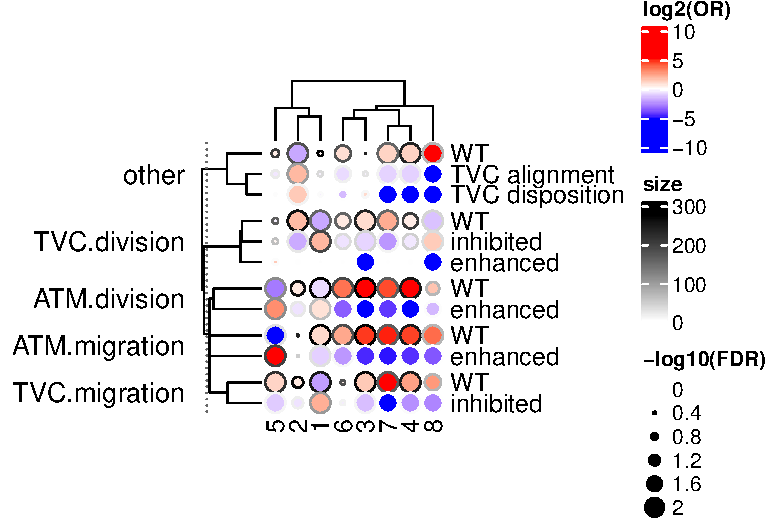
\includegraphics[width=\textwidth]{clust.pheno.pdf}
		\caption{}
		\label{}
	\end{subfigure}
	\caption{(a) Workflow for cluster selection. 
		(b) Optimization of $\gamma$ for $k = 17$. 
		$combined\_score$ is the product of $ES$, $recall$, $log2error$, and $mean\_silhouette$. 
		$ES$ is calculated as in Fig.2b-c, but with interactions ranked by ratio of occurrence within clusters to occurrence between clusters. 
		$recall$ is the fraction of known interactions recovered by creating a gene network using partial modularity between conditions (see equation (5)). 
		$log2error$ gives the result of the reduced $k$-NN classifier.
		$mean\_silhouette$ gives the mean silhouette width as described in equation (6).
		$/nclust$ shows the effect of $\gamma$ on the number of clusters.
	(c) Clusters for optimal combined statistic at $k = 17$ and $\gamma = 0.3266$.
(d) Hypergeometric test for enrichment of conditions in each cluster as given in equations (7-8). 
(e) Enrichment test for experimenter-labeled phenotypes in each cluster.}
	\label{}

\end{figure}

\section{Methods}

\subsection{Preprocessing}

Segmentation of confocal images was performed using Imaris. Summary statistics were extracted for segmened cells in each embryo. From the cell segmentation statistics 116 embryo-level parameters were computed. Parameters were normalized by z-score then scaled between -1 and 1.

\subsection{Dimension Reduction}

Many parameters are strongly correlated (Fig. 2b). This is undesirable because each parameter additively contributes to distance used for clustering, resulting in disproportionate weight being given to phenotypes captured by multiple parameters. Linear methods of dimenison reduction (e.g. PCA) assume that all variables are independent and can be linearly combined. We could not assume that all of our measured input parameters were independent, so we instead used an autoencoder for dimension reduction.

An autoencoder is a neural network architecture widely used for denoising and image recognition. It works by encoding the input data into a lower dimensional representation that can be decoded with minimal loss. By extracting this lower dimensional encoding (the ``bottleneck'' or ``embedding'' layer), an autoencoder can be used for dimension reduction\cite{WANG2016232}. This results in an embedding that corresponds to the information content of the input data rather than absolute distance in phenotype space.

We trained four autoencoders using embedding layers of 2, 3, 7, and 14 dimensions. We selected the 2-dimensional embedding based on Akaike Information Criterion\cite{cavanaugh2019akaike} (Table 1; Fig. 1a), defined as 
\begin{equation}
AIC = 2k - 2ln(\hat{L}) 
\end{equation}
where $k$ is the number of parameters and $\hat{L}$ is a likelihood function, which we define as $1 - MSE$.

\subsection{Clustering Algorithm}
Euclidean distance between embeddings is used to compute a k-nearest neighbors graph. The graph is then partitioned into clusters by modularity\cite{PhysRevE.74.016110}, which is defined as 
\begin{equation}
 \mathcal{H} = \frac{1}{2m}\sum_{c}( \,e_c - \gamma\frac{K_c^2}{2m}) \, 
\end{equation}
 where $m$ is the average degree of the graph, $e_c$ is the number of edges in cluster $c$, and $K_c$ is the number of nodes in cluster $c$. This equation has a nicely intuitive interpretation. Modularity $\mathcal{H}$ of a graph is given by the sum of how well-connected its clusters are, defined as the difference between the number of edges in the cluster and the expected number of edges given the number of nodes in the graph and average degree of a node.

Because optimizing modularity is NP-hard, we used the leiden algorithm to approximate an optimal solution\cite{traag2019louvain}.

Though modularity ensures that clusters are well-connected, the number of clusters returned is dependent on $\gamma$, which cannot be inferred from the data. A value of $k$ must also be selected for the input graph.

\subsection{Hyperparameter Selection}

We performed clustering for 100 random $\gamma$ values between 0.01 and 3.0 for $k$ values ranging from 3 to 53.

We selected $k$ and $\gamma$ based on four validation metrics. Mean silhouette width was calculated from the euclidean distance etween embryos.

\subsubsection{$k$ Selection}
\paragraph{Ortholog Lookup}
We used STRINGdb to construct a known protein interaction network of the perturbed genes\cite{10.1093/nar/gkq973}. Because the \textit{C. robusta} network is poorly characterized, we used ENSEMBL to obtain orthologs from \textit{M. musculus} and \textit{H. sapiens}. 

\paragraph{GSEA}
The known protein interactions can be treated as a gene set for GSEA\cite{subramanian2005gene}. Interactions can be ranked by edge count between embryos in two conditions. An enrichment score is calculated based on occurrence of known interactions near the top of the ranked list. An optimal k can be selected by maximizing enrichment score.

\paragraph{Gene Network}
A gene network can be created from the $k$-NN graph by drawing an edge between a pair of conditions if the $k$-NN graph is enriched in edges between embryos in that pair of conditions.
For each condition pair $(x,y)$, we use a hypergeometric test for enrichment of edges from embryos in $x$ to embryos in $y$.
We assume the null probability $p_{xy}$ to be given by
\begin{equation}
p_{xy}k = \frac{\binom{K_y}{k}\binom{M-K_y}{K_x-k}}{\binom{M}{K_x}}
\end{equation}
where $K_y$ is the total degree of all nodes in $y$, $k$ is the number of edges from nodes in $x$ to nodes in $y$, $M$ is the total degree of all nodes in the graph, and $K_x$ is the total degree of all nodes in $x$. 
Effectively this means we consider all edges to be a population that the edges from nodes in $x$ are drawn from, and look for overrepresenation of edges connected to nodes in $y$. We consider a false disctovery rate of 0.05 to be significantly enriched. 
We define the odds ratio $OR_{xy}$ as
\begin{equation}
OR_{xy} = \frac{\frac{k}{K_x-k}}{\frac{K_y}{M-K_y}}.
\end{equation}
\subsubsection{$\gamma$ Selection}
After selecting a $k$-NN graph, clustering is performed for randomized $\gamma$ values. Four metrics are calculated for each clustering: $log2(error)$, enrichment score, recall, and mean silhouette width. $\gamma$ is selected by optimizing for the product of these values.
\paragraph{Reduced $k$-NN classifier}
A reduced $k$-NN classifier was created from a subset of the embeddings using the clusters as labels. The remaining embeddings were used as a test set. This process was repeated 1000 times per clustering to obtain a mean error.

\paragraph{GSEA}
Condition pairs for each clustering were ranked by the proportion of edges that were between embryos in the same cluster vs. between embryos in different clusters. An enrichment score can be calculates as with $k$ selection.

\paragraph{Comparison to Known Protein Interactions}
A second gene network was constructed using partial modularity between pairs of conditions. We define the partial modularity $H_{xy}$ of a condition pair $(x,y)$ as 
\begin{equation}
 \,H_{xy} = \,e_{xy} - \gamma\frac{\,K_x\,K_y}{2M} \, 
\end{equation}
where $e_{xy}$ is the total number of edges from embryos of condition $x$ to embryos of condition $y$, $K_x$ is the total degree of all embryos of condition $x$, $K_y$ is the total degree of all embryos in condition $y$, and M is the total degree of all nodes in the graph. If $H_{xy}$ is positive, we draw an edge between genes $x$ and $y$. We then calculate a recall score by comparing this graph to the graph of known protein interactions.

\paragraph{Mean Silhouette Width}
Pointwise silhouette width\cite{ROUSSEEUW} $s(i)$ is given by 
\begin{equation}
s(i) = \frac{b(i) - a(i)}{max\{a(i),b(i)\}}
\end{equation}
where $a(i)$ is the average distance between node $i$ and other nodes in the same cluster, and $b(i)$ is the average distance between $i$ and other nodes in the closest other cluster.

\subsection{Cluster Characterization}
\subsubsection{Hypergeometric Test}
We tested for enrichment of experimental perturbations and experimenter-labeled phenotypes in each cluster using a hypergeometric test. For each condition $c$ in each cluster $x$, we assume the probability $p_{xc}$ of the intersect between $c$ and $x$ is given by
\begin{equation}
p_{xc}k = \frac{\binom{n_c}{k}\binom{N-n_c}{n_x-k}}{\binom{N}{n_x}}
\end{equation}
where k is the number of embryos in both $x$ and $c$, $n_c$ is the number of embryos in $c$, $N$ is the total number of embryos, and $n_x$ is the total number of embryos in $x$.

We define the odds ratio $OR_{xc}$ as
\begin{equation}
OR_{xc} = \frac{\frac{k}{n_x-k}}{\frac{n_c}{N-n_c}}.
\end{equation}

\bibliographystyle{plain} % We choose the "plain" reference style
\bibliography{refs} % Entries are in the refs.bib file
\end{document}
